\subsection{Kommunikationsbus}

Til projektet bruges to forskellige typer bus. Mellem DevKit8000 og PSoC-Master benyttes SPI, og mellem PSoC-Master og de tre andre PSoCs (XY, Z og Sensor), samt mellem PSoC-Sensor og nogle af vores sensorer benyttes I2C.

Denne konfiguration er valgt, fordi det kunne være interessant at prøve at bruge mere end én type bus, og fordi det giver en fornuftig afkobling mellem brugerinterfacet på DevKit8000 og resten af systemet. Denne afkobling kunne derefter, i en videreudvikling af systemet, konverteres fra SPI til en form for wireless kommunikation – for eksempel Wifi eller Bluetooth.

\subsubsection{Serial Peripheral Interface (SPI)}

Serial Peripheral Interface (SPI) er en 4-wire, seriel data bus, der understøtter fuld duplex kommunikation mellem en enkelt master enhed og flere slave enheder.

Hardwaremæssigt kræver SPI fire ledninger fra master enheden til slave enhederne (der findes også specielle konfigurationer med færre ledninger, men dem kommes der ikke ind på her):

\begin{itemize}
    \item SCLK - Serial clock
    \item MISO - Master In, Slave Out
    \item MOSI - Master Out, Slave In
    \item SS - Slave Select (active low)
\end{itemize}

De første tre linjer er fælles for alle enheder på bussen, mens der skal være en Slave Select per slave der skal kunne adresseres.

Selve kommunikationen foregår ved at master vælger en slave ved at sætte slavens SS lav, og derefter sender master taktslag på SCLK. For hvert taktslag bliver der overført en bit fra master til slaven i MOSI, og en bit fra slaven til master i MISO. Dette foregår typisk ved hjælp af skifteregistre, arrangeret så de former en ringbuffer.

\begin{figure}[H] \centering
    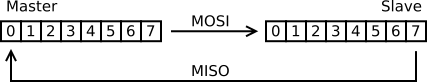
\includegraphics{0_Filer/Figuer/5_HW_Design/SPI_ringbuffer.png}
    \caption{SPI skifteregister ringbuffer}
    \label{fig:HWD_SPI_ring}
\end{figure}

Da kommunikationslinjerne er delte kræver det, at alle slaver på bussen ignorere data på SCLK og MOSI, og holder MISO som høj impedans så længe deres SS er inaktiv – dvs. så længe master enheden ikke har udvalgt dem.

SPI kommunikation har flere fordele:

\begin{itemize}
    \item Fuld duplex
    \item Meget simpel adressering – sæt et signal lavt, ingen behov for at bruge tid på at sende adresser
    \item Meget simpel protokol – ingen formelle krav om formattering, kan sende data med vilkårlige bitlængder
    \item Høj hastighed
\end{itemize}

Men der er også nogle ulemper ved SPI:

\begin{itemize}
    \item Adresseringen bruger et kabel, og en IO pind på master, per slave (kan undgås med daisy-chaining, men det øger kompleksiteten af protokollen og stiller krav til slavernes opførsel)
    \item Den meget simple protokol giver ingen hjælp til detektion af eller robusthed overfor fejl.
    \item Kun master enheden kan starte kommunikationen – hvis en slave vil sende noget til master enheden, må den vente på at masteren initierer, og slaver kan slet ikke kommunikerer med hinanden direkte.
\end{itemize}

\subsubsection{Inter-Integrated Circuit (I2C)}

Inter-Integrated Circuit (I\textsuperscript{2}C eller I2C) er en 2-wire, seriel bus, der understøtter halv duplex kommunikation mellem flere enheder – i princippet er alle enheder lige i I2C, men i praksis vil de oftest være delt ind i masters og slaver ligesom i SPI, dog med den undtagelse at I2C understøtter flere masters på en bus og at enheder kan skifte roller.

Hardwaremæssigt kræver I2C kun to ledninger, der er delt mellem alle enheder på bussen. Dog skal de begge have en pull-up modstand, så de bliver holdt høj, når de er idle. De to linjer er:

\begin{itemize}
    \item SCL - Serial Clock Line
    \item SDA - Serial Data Line
\end{itemize}

\begin{figure}[H] \centering
    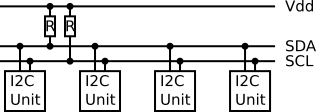
\includegraphics{0_Filer/Figuer/5_HW_Design/I2C_opsaetning.png}
    \caption{Eksempel på I2C kredsløb}
    \label{fig:HWD_I2C_kreds}
\end{figure}

I I2C følger kommunikationen en fast protokol, hvor den enhed der gerne vil initiere kommunikationen (master) først signalerer en start sekvens, og derefter sender data på SDA mens SCL laver et taktslag for hver bit. For at sørge for at der ikke kommer nogen falske aflæsninger af data, så er konventionen at SDA sætter det ønskede niveau på SCL falling-edge, og at SDA aflæses på rising-edge.

Den data der sendes er også underlagt en fast protokol: Den første byte, der bliver sendt skal bestå af først en 7-bit adresse på den enhed, som masteren gerne vil kommunikerer med (slaven), efterfulgt af en læse/skrive bit (0 = skrive til slaven, 1 = læse fra slaven). Derefter begynder den skrivende enhed at sende data på SDA i hele bytes, mens master enheden holder takten på SCL. Desuden bliver der, gennem hele forløbet transmitteret en acknowledge bit af den modtagende enhed efter hver hele byte der bliver modtaget.

Til sidst, når master enheden syntes at kommunikationen er færdig, laver master en stop sekvens, der frigiver bussen så en anden enhed kan komme til.

Et par eksempler på hvordan protokollen kører (hvide felter skrives af master, grå af slave):

\begin{figure}[H] \centering
    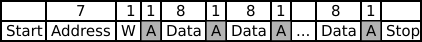
\includegraphics{0_Filer/Figuer/5_HW_Design/I2C_Write.png}
    \caption{I2C Master skriver til slave}
    \label{fig:HWD_I2C_write}
\end{figure}

\begin{figure}[H] \centering
    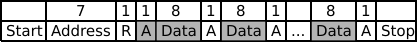
\includegraphics{0_Filer/Figuer/5_HW_Design/I2C_Read.png}
    \caption{I2C Master læser fra slave}
    \label{fig:HWD_I2C_read}
\end{figure}

\begin{figure}[H] \centering
    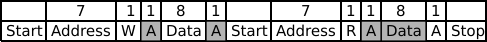
\includegraphics{0_Filer/Figuer/5_HW_Design/I2C_Mixed.png}
    \caption{I2C Master skriver en byte til, derefter læser en byte fra slave}
    \label{fig:HWD_I2C_blandet}
\end{figure}

Figur \ref{fig:HWD_I2C_blandet} giver et eksempel på hvordan en sammenhængende kommunikation kan have data i begge retninger, uden at bussen frigives imellem ændringerne i dataflow retningen.

De umiddelbare fordele ved I2C er:

\begin{itemize}
    \item Understøttelse for flere master enheder
    \item Software addressering er fleksibel
    \item Det kræver ikke ekstra kabler eller IO pins at sætte en ekstra enhed på bussen
    \item Alle enheder kan tale direkte med hinanden
    \item Byte-ACK protokollen sikre den overordnede integritet af kommunikationen
\end{itemize}

Men I2C har også nogle ulemper og begrænsninger:

\begin{itemize}
    \item Ingen fuld duplex
    \item Lav hastighed i forhold til SPI
    \item Byte-ACK protokollen giver meget ringe beskyttelse overfor bit-fejl og generel data korruption.
\end{itemize}
